\chapter{Tail loss?}

\section{Introduction}


Chordates are composed of three subphyla\textemdash vertebra, tunicata and cephalochordata\textemdash that all share several characteristics, the notochord being the key characteristic, which is indicative of the phyla name. The tail development of larvacean (Oikopleura) and several species of ascidians, tunicates have been studied \cite{jeffery_factors_1992,nakatani_mutations_1999,kugler_evolutionary_2011}. Larvacean form tailed larvae with a hollow dorsal notochord and keep their tail throughout their adult life stage, ascidians form their tail in similar manner before undergoing the process of metamorphosis, where the larval tail is absorbed in to the trunk region \cite{paris_history_2008}. A typical ascidian larvae tail forms through the convergence, intercalation and extension of the notochord and the differentiation of the posterior muscle cells \cite{swalla_mechanisms_1993}. When fully formed the ascidian notochord contains 40 cells, flanked by three rows of muscle. The ancestral notochord or notochord-like structure is believed to have been muscle based, this is perhaps the reason behind the tail formation being tied to both notochord and muscles \cite{lauri_development_2014}. This is not a far fetched idea seeing that the primary and secondary notochord and muscle lineage are derived from the same blastomere, and the ascidian tail needs both the notochord and differentiated muscle to form a larval tail \cite{nishida_cell_1987,di_gregorio_tail_2002}.

Of the \mytilde3000 species of ascidians less than 20 have been identified as independently undergoing tail-loss, with the majority being Molgulide species \cite{berrill_studies_1931,huber_evolution_2000}. Although the mechanism behind tail-loss differs by species, a common characteristic is the lack of a notochord that intercalates and extends, and undifferentiated muscle cells\cite{swalla_mechanisms_1993}. \textit{M. bleizi} notochord cells converge to the midline, and began to extend, however, cells never properly intercalated and the tail formation stop before it is fully formed \cite{jeffery_evolution_1999}. In \textit{M. bleizi} there is an early down-regulation of \textit{brachyury} (\textit{bra})\textemdash a key notochord inducer\textemdash and larva-specific muscle actin genes (\textit{MbMA}) have become pseudo genes.   

A similar process was observed in \textit{M. occulta}, muscle actin becoming pseudo genes, however, the mutations were not the same \cite{}. \textit{M. occulta} and \textit{M. oculata} are two closely related species, who in their adult form are virtually identical, with the exception of a white pigment spot between the two siphons of the tailed species, \textit{M. oculata}. During development the species are indistinguishable up to the gastrula stage. It is at late gastrula when the notochord and muscle cells begin to move posteriorly \cite{swalla_novel_1993}. There are several steps that take place to form the notochord and tail; first the notochord cells move mediolaterally to the midline, next the cells polarize and intercalate, changing their shape and extending posteriorly \cite{keller_mechanisms_2000, jiang_ascidian_2005,stemple_structure_2005}. This process is known as convergence and extension. 

Several key tail development genes have been identified as present in \textit{M. occulta}, but not expressed at a sufficient level \cite{swalla_interspecific_1990,jeffery_factors_1992,swalla_novel_1993}. With advances in high throughput sequencing technologies, gene expression of \textit{M. occulta}, \textit{M. oculata}, and hybrid species can be analyzed on a whole transcriptome level \cite{gyoja_analysis_2007,pickrell_variation_2010}. mRNA of three different developmental stages for \textit{M. occulta}, \textit{M. oculata}, and their hybrid have been sequenced and assembled at Michigan State University (MSU). The three transcriptomes were used to identify the presence or absence of known notochord genes downstream of bra using C. intestinalis data from the NCBI database. BLAST searches were with known notochord genes, and several of them were selected for further analysis. FGF9/16/20, prickle (pk), and several other downstream \textit{bra}, to construct a \textit{brachyury} gene regulatory network for both \textit{M. occulta} and \textit{M. oculata}. 
Simple body plan with a small number of cells \cite{satoh_ascidian_2001,satoh_genome_2002}, rapid embryo development.

Induced at the 32 cell stage by \textit{FGF9/16/20}
muscle and notochord come from the same cell lineage.
Hybrids are tails are resorted in embryos that contain p58, which stains in the muscle 
It is thought that the early form of the notochord where not cartilage based but were made of muscle.   

----

\section{Methods}
\subsection{Sample collection, sequencing and assembly}
DNA was extracted from the gonads of an individual adult specimen for %\textit{M. occidentalis},
\textit{M. occulta}, and \textit{M. oculata}. Three paired-end jumping libraries were collected for each species ranging from \mytilde300bp to \mytilde950bp. Further details about extraction methods and libraries can be found in Stolfi et al., \cite{stolfi_divergent_2014}. RNA was extracted from all three \textit{Molgula} species using the methods discussed in Lowe et al., \cite{}. RNA for the gastrula (3hpf), neurula (4hpf) and mid-tailbud (6hpf) stages were extracted for both \textit{M. occulta} and \textit{M. oculata}, with a replicate for the gastrula and a sample for early-tailbud stage sequenced from \textit{M. occulta}. %Samples from a fertilized embryo, tailbud and larvae were sequenced for \textit{M. occidentalis} to gain a broad scope of expression. 
Sequencing for \textit{M. occulta} and \textit{M. oculata} RNA were conducted at the Michigan State University, well all other sequencing was done at New York University. All libraries were paired-end, with 75 base pair (bp) reads for the sequencing done at MSU and 100 bp reads for the NYU sequencing. 

Genome assemblies were conducted using 3-pass digital normalization \cite{brown_reference-free_2012} and assembled using Velvet\cite{zerbino_velvet:_2008}. Other assemblers were tested, however, Velvet produced the best results by having the least fragmented assemblies. Assemblies were initially done with 21 $\geq$ k $\/eq$ 71, for intervals of 10. Assemblies were selected for which `k' produced the highest N50, than species were reassembled for a k$\pm$10 with a step size of 2 of the selected assembly. A k of 31, 49, and 37 were select for \textit{M. occulta}, \textit{M. oculata}, and \textit{M. occidentalis}, respectively. 

Both \textit{de novo} and reference based assembly were used to create gene models. Reads were mapped to their respective genomes using bowtie2 and tophat to identify genes and alternative splicing variants \cite{langmead_fast_2012,trapnell_differential_2012}. The accepted.bam files were then sorted and indexed using samtools \cite{li_sequence_2009}. The sorted bam files where then processed using cufflinks and cuff merge to generated consensus gtf annotation files. The digitally normalized trinity \textit{de novo} assembled transcripts from Lowe et al., were aligned to their respective genomes using BLAT \cite{haas_novo_2013}. The cufflinks/cuffmerged gtf files were then converted into bed files and merged with the annotation files from the mapped \textit{de novo} assembled aligned using gimme (https://github.com/likit/gimme). Gimme joins gene models using a graph based method to develop more complete transcripts. The gimme gene models were then converted to gff format using the script bed2gff in the gimme utils folder in order to extract the transcripts from the genome in a multi pasta file. Transcripts were then extracted using ``gffread -w transcripts.fa -g /path/to/genome.fa transcripts.gtf'' which is included in the cufflinks package. The extracted transcripts were then partitioned into transcript families and annotated using khmer suite and steps found in the eel-pond protocol \cite{}. \textit{Ciona intestinalis} was used as a reference, and the sequences were retrieved as discussed in Chapter 3. 

\subsection{Gene counts and differential expression analysis}
Reads were mapped to transcripts from the gimme gene modules for their respective species. Hybrid reads are mapped onto the \textit{M. occulta} and \textit{M. oculata} transcripts as well, seeing that they are F1 hybrids and should contain an allele from each parent. Read counts were generated using express \cite{}. Express gives the option of ``Total counts'' and ``Effective counts'', which reports the number of reads mapped per transcript and the normalized counts based on transcript length, respectively. Because EdgeR insist on unnormalized reads, ``Total counts'' were used. A replicate was only provided for one of the samples, 3hpf, because of this various dispersion calculation methods were used. the one replicate was used to calculated statistics, in addition to 5hpf being treated as a replicate for 6hpf. These time points represent what would be early and mid-tail bud stages in the urodele ascidian. 

\section{Results}
\subsection{\textit{M. occulta} and \textit{M. oculata} have strong overlap in gene presence}
\textit{C. intestinalis} is the closest ascidian species with a well annotated gene, because of these reason it was used to annotate the genomes of both \textit{M. occulta} and \textit{M. oculata}. Reciprocal best hit (RBH) blast with an e-value of 1e-3, were done with the \textit{M. occulta} and \textit{M. oculata} transcriptomes against \textit{C. intestinalis} for the annotation of both species.  We are aware this is a low threshold for homologue, however, seeing that on a large-scale, information for these species are not known and we wanted to gain any possible insight go the composition of the genes present in each species. The gene models for \textit{M. occulta} and \textit{M. oculata} produced 42,365 and 40,775 sequences total, respectively. \textit{M. occulta} 8627 annotated / ortho 22700 annotated / homolog \textit{M. oculata} 8,677 annotated were orthologs, 22,583 were annotated homologs. \textit{M. occulta} and \textit{M. oculata} have a high overlap in number of translated transcripts that showed any level of homology with \textit{C. intestinalis} proteins from the NCBI database. Of the 16,414  proteins \textit{M. occulta} had BLAST hits for 83.6\% and 86.5\% had hits in \textit{M. oculata}. \textit{M. occulta} had hits for 453 proteins that were not found in \textit{M. oculata} and \textit{M. oculata} had hits for 921 transcripts that did not have hits in \textit{M. occulta}, overlapping by 97\%.

\begin{figure}[tbp]
\centering
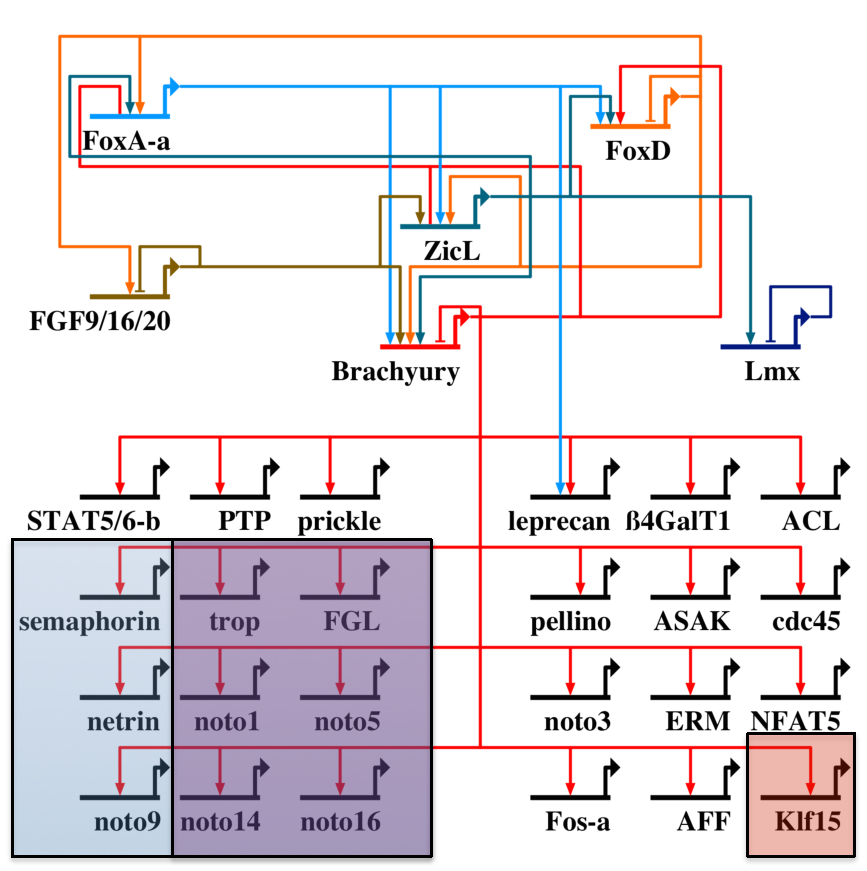
\includegraphics[scale=0.55]{figures/bra_grn.pdf}
\caption{\textbf{\textit{Brachyury gene regulatory network} }}
\label{fig:bra_grn}
\end{figure}
\subsection{Notochord gene network}

Next, we examined genes associated with notochord development in \textit{C. intestinalis} to better analyze the molecular development of the tail. Genes were identified as being involved in tail formation and notochord development, by interactions with \textit{bra} with a strong focus on downstream \cite{hotta_temporal_1999,hotta_characterization_2000,hotta_brachyury-downstream_2007,kugler_evolutionary_2008,kugler_evolutionary_2011}. From these studies many potential notochord genes were identified, we compiled a list of 67 genes and identified there presence or absence within the genomes and transcriptomes of both \textit{M. occulta} and \textit{M. oculata} (Figure~\ref{fig:bra_grn}). Of the 67 genes 11 were missing from the transcriptomes of both species, those genes were, \textit{cofilin}, \textit{entactin} (\textit{nidogen-2-like}), \textit{fibrinogen-like protein} (\textit{FGL}), \textit{fibronectin}, \textit{multidom}, \textit{noto1}, \textit{noto5}, \textit{noto14}, \textit{noto16}, and \textit{tropomyosin}. Of the remaining genes without orthologus sequences were \textit{netrin}, and \textit{noto9} in \textit{M. occulta} and \textit{Klf15} in \textit{M. oculata}. In \textit{Ciona} \textit{netrin} stains in the notochord and the central nerves system and is associated with axon guidance\cite{hotta_characterization_2000}. \textit{Klf15} was identified to be in the notochord, but there is currently no know function associated with the gene \cite{passamaneck_direct_2009}. This shows a strong overlap in the number of notochord associated genes present in both species.

\subsection{Differential expression between neurala and tailbud appears to be key factor is tail development} 

\begin{table}[b]
\caption{Differential expression: Species \textit{vs} time}
\makebox[\linewidth]{
\centering
\begin{tabular}{l c c c c}
\hline\hline
{\multirow{2}{*}{Species} } & {\multirow{2}{*}{Condition} }&\multicolumn{3}{c}{Number of transcripts that show...} \\ %\cline{1-6}% inserts table %heading
& & Up-regulation & Down-regulation & No differential expression \\ [0.5ex]
\hline
{\multirow{2}{*}{\textit{M. occulta} }} 	&						
Gastrula \textit{vs} Neurula& 260 & 8 & 20197  \\ 
\multicolumn{1}{ c  }{}                        			&				
Neurula \textit{vs} Tailbud&1 & 4 & 20460    \\ \cline{1-5}
{\multirow{2}{*}{\textit{M. oculata} }} &
Gastrula \textit{vs} Neurula& 119 & 66 & 20280  \\ 
\multicolumn{1}{ c  }{}                        &
Neurula \textit{vs} Tailbud&1170 & 626 & 18669    \\ \cline{1-5}
{\multirow{2}{*}{Hybrid }} &
Gastrula \textit{vs} Neurula& 21 & 99 & 20345  \\ 
\multicolumn{1}{ c  }{}                        &
Neurula \textit{vs} Tailbud&1270 & 129 & 19066    \\ 
\hline
\end{tabular}
\label{table:de}
}
\end{table}

The down regulation of \textit{manx} and \textit{58} amongst other genes were shown to be one of the causes behind the tail loss in \textit{M. occulta}, because of this we know tail formation is tied to differential expression. We sequenced and assembled three developmental stages\textemdash gastrula, neurula, and tailbud\textemdash across \textit{M. occulta}, \textit{M. oculata} and their hybrid. The tail-less species, \textit{M. occulta}, showed the highest level of differential expression, with 260 (97\%) of the transcripts said to be differentially expressed were up-regulated (Table~\ref{table:de}). \textit{M. oculata} also had more transcripts being up-regulated (65\%) than down. Hybrids did not follow this trend; the major of its genes were being down-regulated (82\%).  

When comparing the neurula stage to the tailbud stage there was essentially no significant differential expression observed in \textit{M. occulta}. A total of 5 genes were said to be differentially expressed (FDR < 0.05). However a major shit in differential expression occurred when comparing both \textit{M. oculata} and the hybrid for these conditions (Figure~\ref{fig:de_plots}). There were 1170 and 1270 genes up-regulated, and transcripts and 129 transcripts down-regulated for \textit{M. oculata} and the hybrid respectively. That equates to a 10\textit{x} increase in differentially expressed transcripts in both hybrid and \textit{M. oculata}.


\begin{sidewaysfigure}[!ht]
	\subfloat[\label{subfig-1:mocc3v4}]{%
	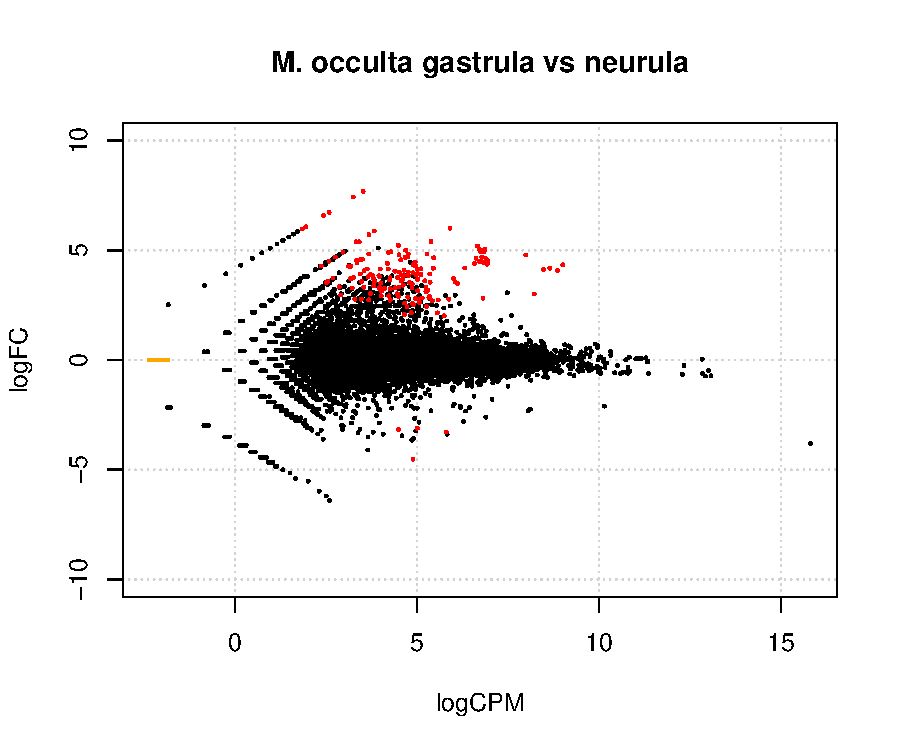
\includegraphics[scale=0.5]{figures/mocc3v4_graph.pdf}
	}
	\subfloat[\label{subfig-2:mocu3v4}]{%
	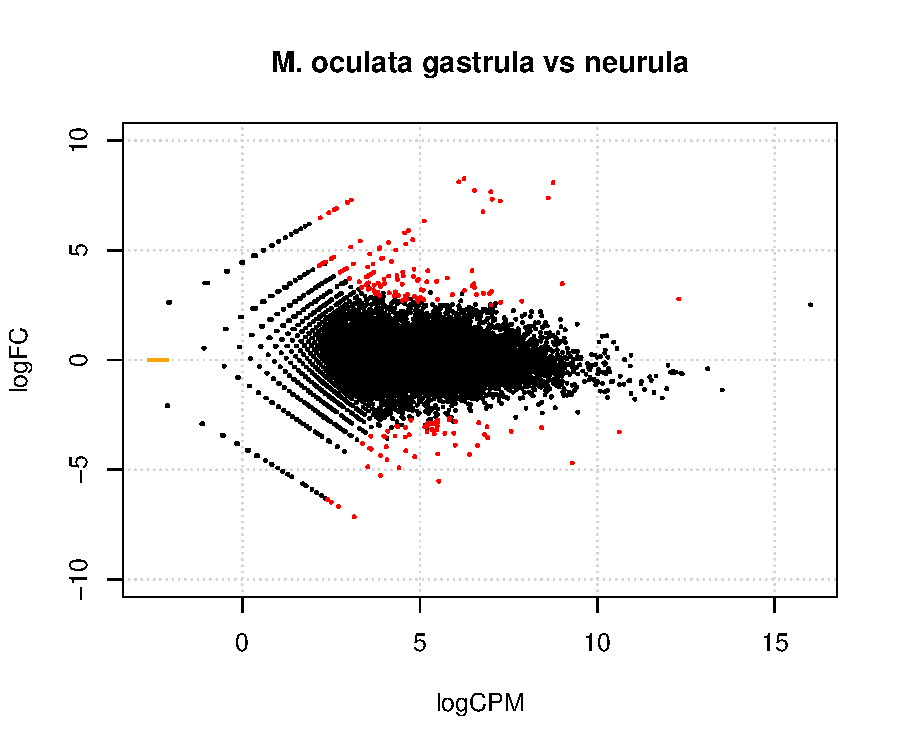
\includegraphics[scale=0.5]{figures/mocu3v4_graph.pdf}
	}
	\subfloat[\label{subfig:hyb3v4}]{%
	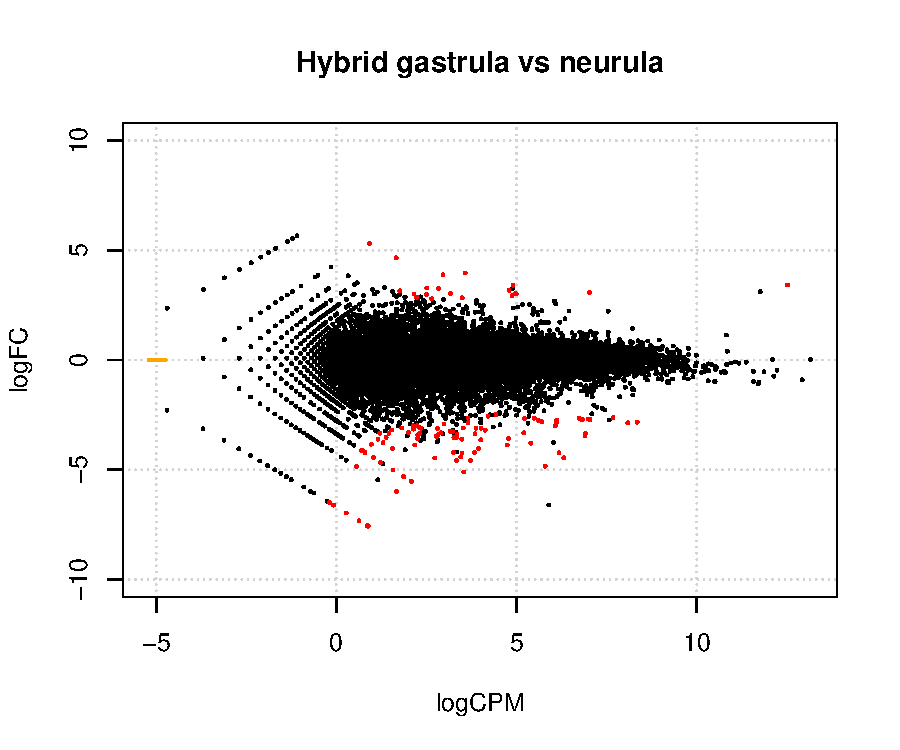
\includegraphics[scale=0.5]{figures/hyb3v4_graph.pdf}
	}
	\hfill
	\subfloat[\label{subfig:mocc4v6}]{%
	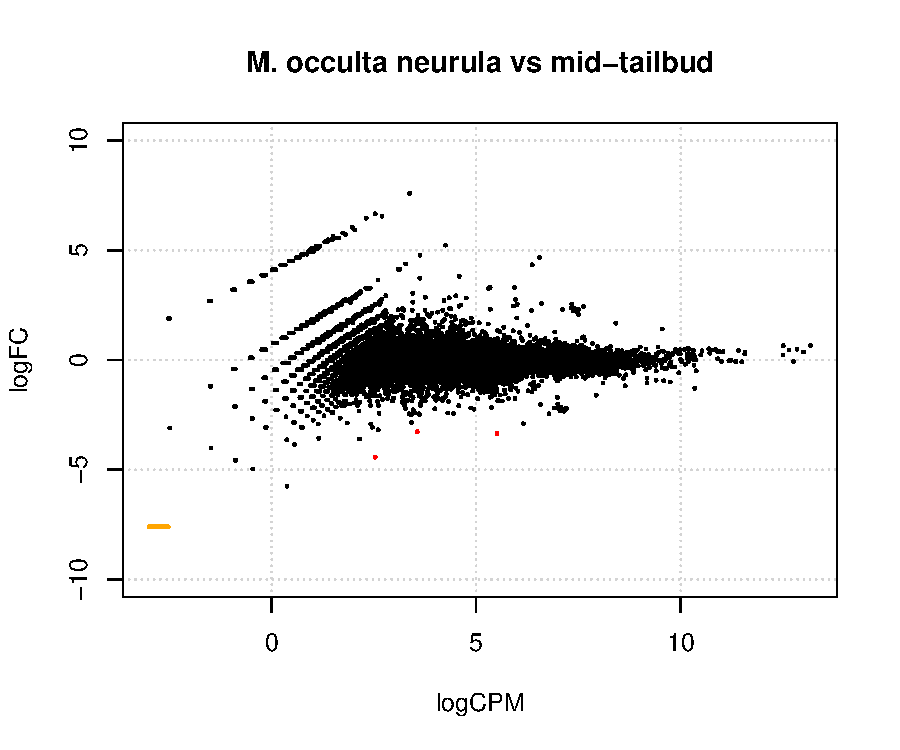
\includegraphics[scale=0.5]{figures/mocc4v6_graph.pdf}
	}
	\subfloat[\label{subfig:mocu4v6}]{%
	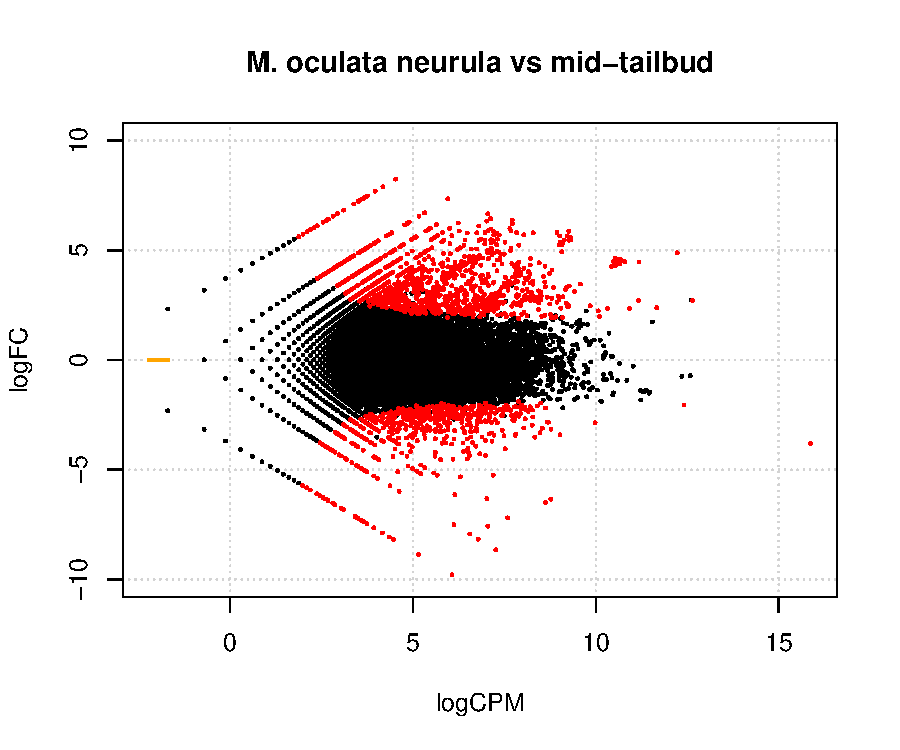
\includegraphics[scale=0.5]{figures/mocu4v6_graph.pdf}
	}
	\subfloat[\label{subfig:hyb4v6}]{%
	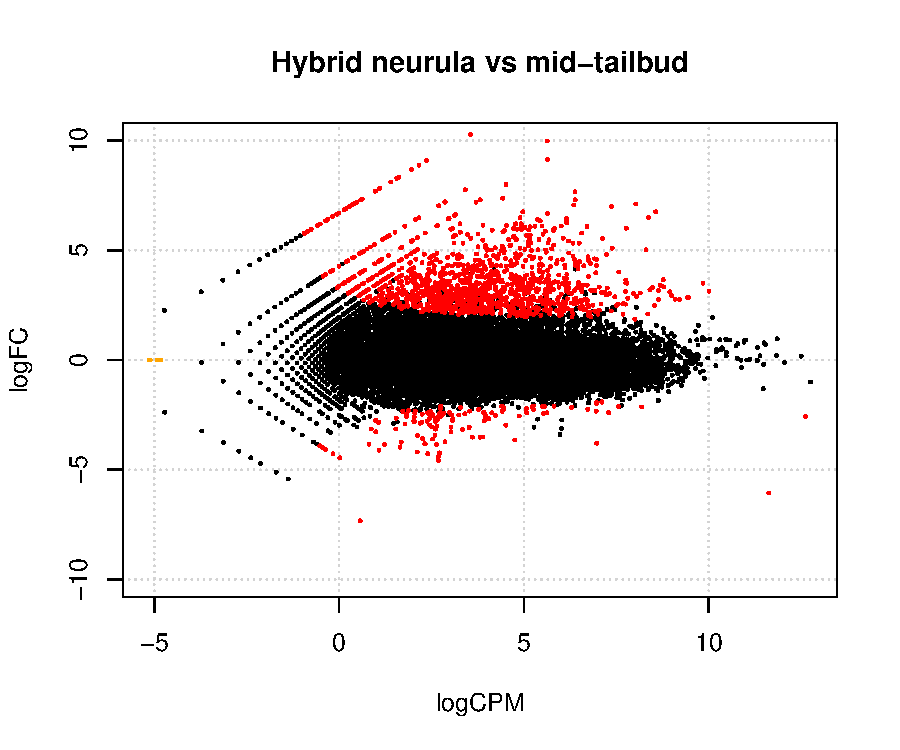
\includegraphics[scale=0.5]{figures/hyb4v6_graph.pdf}
	}
	\caption{\textbf{Differential expression of homologous transcripts.} The k-mer distribution is shown for each assembler and assembly condition, diginorm (DN) and unnormalized reads. The k-mer distribution is the coverage of a given k-mer verses how many k-mers of that coverage is incorporated in the respective assemblies. Both Oases and Trinity assemblies are shown for ~\ref{fig:figure_2_Mocc_dist} \textit{M. occulta} k-mer distribution and  ~\ref{fig:figure_2_Mocu_dist} \textit{M. oculata} k-mer distributions. Trinity had a higher k-mer distribution for both species, reflective of the inclusion of more low abundance reads into the Trinity assemblies.}
	\label{fig:de_plots}
\end{sidewaysfigure}

\subsection{Overlap between hybrid and M. oculata allele }
When comparing transcript expression at neurula stage and tailbud stage \textit{M. oculata} and the hybrid has a total of 2,440 transcript up-regulated between the two of them. Of that 2,440 transcripts 328 (13\%) overlap (Figure~\ref{fig:overlap}. There were no transcripts for \textit{M. occulta} that were also identified as differentially expressed. Of the transcripts that were down regulated, there was only an overlap of 5 transcripts (0.06\%) between \textit{M. oculata} and the hybrid, and none between \textit{M. occulta}. We wanted to take a closer look at these transcripts so we also examined the allele specific expression to determine if the \textit{M. oculata} or \textit{M. occulta} was influencing the expression of these transcripts. 
overlap, large skew for \textit{M. oculata} allele
up-regulated in hybrid but not overlapping, not a drastic difference but still more expression coming from \textit{M. oculata} allele.
general trend for allele differential expression at tailbud 32\% M. oculata, 36\% M. occulta and 32\% hybrid

\begin{figure}[!ht]
	\subfloat[\label{subfig-1:overlap}]{%
	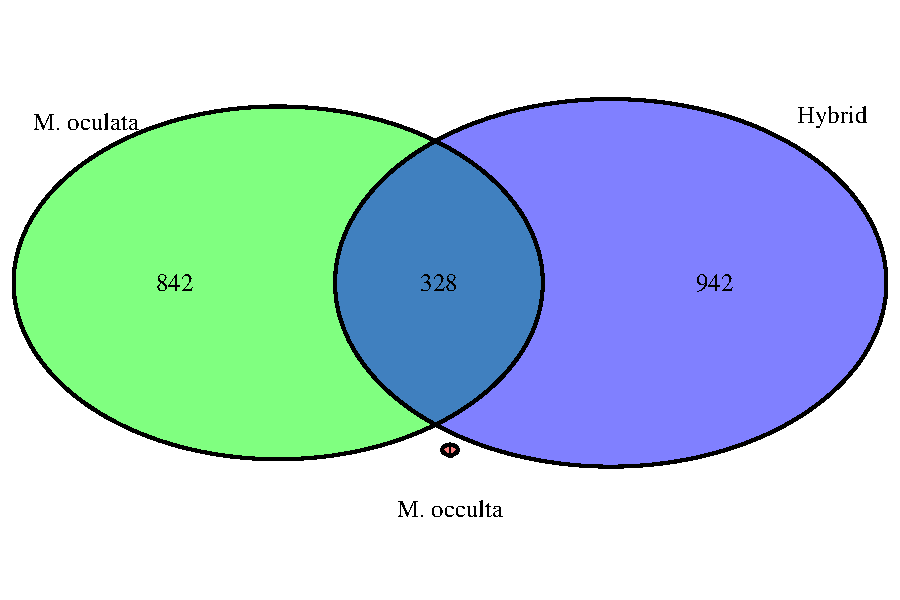
\includegraphics[width=0.45\textwidth]{figures/up_reg.pdf}
	}
	\subfloat[\label{subfig-2:overlap_allele}]{%
	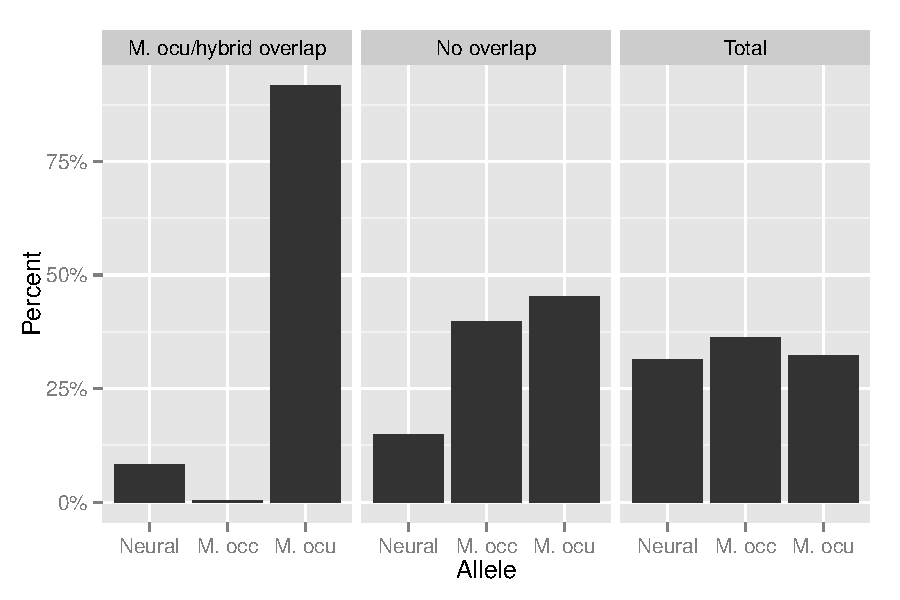
\includegraphics[width=0.45\textwidth]{figures/up_reg_allele_tb.pdf}
	}
	\caption{\textbf{Upregulated transcripts overlap between hybrid and \textit{M. oculata}.} The k-mer distribution is shown for each assembler and assembly condition, diginorm (DN) and unnormalized reads. The k-mer distribution is the coverage of a given k-mer verses how many k-mers of that coverage is incorporated in the respective assemblies. Both Oases and Trinity assemblies are shown for ~\ref{fig:figure_2_Mocc_dist} \textit{M. occulta} k-mer distribution and  ~\textit{M. oculata} k-mer distributions. Trinity had a higher k-mer distribution for both species, reflective of the inclusion of more low abundance reads into the Trinity assemblies.}	
	\label{fig:upreg_tb}
\end{figure}

\section{Discussion}
The genes missing in the Molgulide were also missing in \textit{O. dioica}.
Appears to be a correlation between the up-regulated transcripts in the hybrid and \textit{M. oculata}, 15\% of the genes overlap and none in \textit{M. occulta}. These transcripts may be important for tail formation. Of those transcripts it appears that express is being restored from \textit{M. oculata} allele. 
\section{Conclusion}
